
%%%%%%%%%%%%%%%%%%%% file icsc2017_template.tex %%%%%%%%%%%%%%%%%%%%%
%
% This is the LaTeX source for the instructions to authors using
% the LaTeX document class 'llncs.cls' for contributions to
% the Lecture Notes in Computer Sciences series.
% http://www.springer.com/lncs       Springer Heidelberg 2006/05/04
%
% It may be used as a template for your own input - copy it
% to a new file with a new name and use it as the basis
% for your article.
%
% NB: the document class 'llncs' has its own and detailed documentation, see
% ftp://ftp.springer.de/data/pubftp/pub/tex/latex/llncs/latex2e/llncsdoc.pdf
%
%%%%%%%%%%%%%%%%%%%%%%%%%%%%%%%%%%%%%%%%%%%%%%%%%%%%%%%%%%%%%%%%%%%


\documentclass[runningheads,a4paper]{llncs}

\usepackage{amssymb}
\setcounter{tocdepth}{3}
\usepackage{graphicx}
% \usepackage{url}
\usepackage{hyperref}
\hypersetup{hidelinks}
\usepackage{listings}
%\usepackage{float}
%\restylefloat{figure, lstlisting} 


\newcommand{\keywords}[1]{\par\addvspace\baselineskip
\noindent\keywordname\enspace\ignorespaces#1}

\pagestyle{headings}
% !TeX spellcheck = en_US 

\addtolength{\textfloatsep}{-15px}
\addtolength{\intextsep}{-5px}

\begin{document}

\mainmatter  % start of an individual contribution

% first the title is needed
\title{Frequency Modulation with Feedback in Granular Synthesis}

% a short form should be given in case it is too long for the running head
\titlerunning{FM with Feedback in GS}

\author{\O{}yvind Brandtsegg, Victor Lazzarini}
%

\institute{Norwegian University of Science and Technology, Maynooth University \\ \email{oyvind.brandtsegg@ntnu.no, victor.lazzarini@mu.ie}}



\maketitle

\begin{abstract}

The paper investigates audio synthesis with frequency modulation feedback in granular synthesis, comparing it with regular FM feedback. The combinations of these two classic synthesis techniques show some promising areas of exploration. As a full exploration of this potential is beyond the scope of this paper, we will rather give insight into some initial experiments and share the tools used, encouraging the reader to dive deeper into parameter combinations not yet described.

\keywords{Frequency Modulation, Granular synthesis, Particle synthesis}
\end{abstract}


\section{Introduction}
FM synthesis is one of the classic synthesis techniques, with early explorations by James Tenney, Jean-Claude Risset and John Chowning. A theoretical description was given in \cite{Chowning-73}. FM feedback has more recently been thoroughly investigated by \cite{Lazzarini-2024}. Frequency modulation in granular synthesis has been briefly explored by \cite{Ervik-Brandtsegg} but it is still a relatively lightly explored topic. Here we will look at FM with feedback within granular synthesis as it allows some new means of pitch stabilisation, poses some new problems, and enables some exciting new sonic extensions to both FM and granular synthesis domains.

\section{Basis for comparison}
FM feedback with oscillators and FM feedback in granular synthesis are closely related. Both techniques use a wavetable-reading oscillator to create the output waveform, and the waveform frequency is modulated by the output waveform via feedback. Granular synthesis differ from the simpler oscillator case in that the wavetable-reading process is reinitialized on every grain, and that an envelope is applied to each grain. The envelope applied to grains can be seen as a form of amplitude modulation, with the envelope shape as the modulator waveform. The reinitialization of wavetable reading on each grain also means we can have a periodic phase reset. Phase considerations can have a significant effect on feedback modulation, as we will also see later when we apply a phase delay in the modulation feedback loop.

\subsection{\emph{Basics} for comparison}
To enable a comparison between the two techniques, we have attempted to create parameter settings for the granular synthesizer that as closely as possible resemble the output from a simple oscillator. In that situation, we can compare different parameter settings that apply to both synthesis models. Then, from that comparable situation, we can later apply parameter changes to the granular process that are not available in the simple oscillator model. By doing this, we can explore in specific how the granular model extends the notion of FM feedback in the granular domain. Due to length limitations, the present article will focus on mapping out the similarities.

In granular synthesis, the perceived pitch is constituted by the grain rate (\cite{Roads-2001}, \cite{Brandtsegg-particle}). We have thus chosen to let the grain rate be equal to the fundamental frequency of the simple oscillator. Similarly, it makes sense in the context of comparison to set the grain frequency (reading speed of the waveform inside each grain) equal to this fundamental frequency. With the appropriate envelope, this should allow the granular generator to generate a signal (almost) identical to the simple oscillator. The envelope needs to have a smooth fade in and out, and there need to be sufficient overlap between grains to create a constant amplitude in the output. These constraints can be fulfilled in several different ways. With the constraint that the grain rate should be equal to the fundamental frequency, the options for the envelope are more limited. We have chosen to use a grain duration of 1.5/grainrate, which means that we have a grain overlap of 66\% (the first and last 1/3 of the grain will overlap with neighboring grains). We then use 1/3 of the grain duration for fade in, and equally 1/3 of the duration for fade out. In between fade in and fade out, each grain has a full power sustain period of 1/3 of the grain duration. With an equal power crossfade, we should then be able to recreate a (non granular) waveform. A sigmoid shape is used for the fade in and out of the envelope, to enable equal power crossfading between grains. Changes to the grain duration has significant impact on the resulting sound, and in this case also affects the amount of modulation. Longer grains will give higher amount of modulation, both due to the total energy inserted into the feedback signal, and the amount of time it remains active as a modulation source.

FM feedback with simple oscillators will in its simplest form induce pitch drift, as the output waveform modulate the frequency of the oscillator. This pitch drift can be partly counteracted by recent developments in FM theory (\cite{Lazzarini-2024}), introducing an amplitude modulation component into the feedback path. We will use this as parametric variation when we explore beyond the simplest possible comparisons. The pitch drift can also partly be neutralized by adjusting the phase of the feedback modulator. In feedback modulation, adjusting the phase can be done by introducing a small delay in the feedback signal chain. In digital audio processing the smallest possible feedback delay is 1 sample, so there is inevitably a delay in the feedback in any case. Adjusting the delay time with respect to the fundamental frequency, we attain a similar effect to adjusting the phase of an oscillator which has predictable effects in regular FM synthesis. For this reason, delay times are given in fractions of a cycle of the fundamental frequency in the code examples and experiments shown below.

\subsection{Examples, comparing FM feedback in the two synthesis models}
In our first example we will try to set the parameters so that we get a basic similar, or comparable, sound from both synthesis models. An empirical adjustment to the modulation index for the granular method was needed to better align the two synthesis methods. The effective modulation is dependent on grain duration (as mentioned above). Moreover, the granular model seems to need a slightly different shape of evolution for the modulation index. The empirical formula for modulation index adjustment (written in Csound code here) is thus:  

\begin{lstlisting}
	kmodindex = (kmodindex^1.8)/(kgraindur^0.7) 
\end{lstlisting}

Example 1 uses an increasing modulation index over time. As can be seen in figure \ref{fig:ex1}, the sidebands show a similar evolution. The first sidebands (over the first 1.5 seconds) appear ever so slightly earlier in the oscillator model, but the break to subharmonics (octaviaton) occurs slightly earlier in the granular model (at around 2.5 seconds). The transition to chaotic behavior occurs earlier in the granular model. 

\begin{figure}[h]
	\centering
	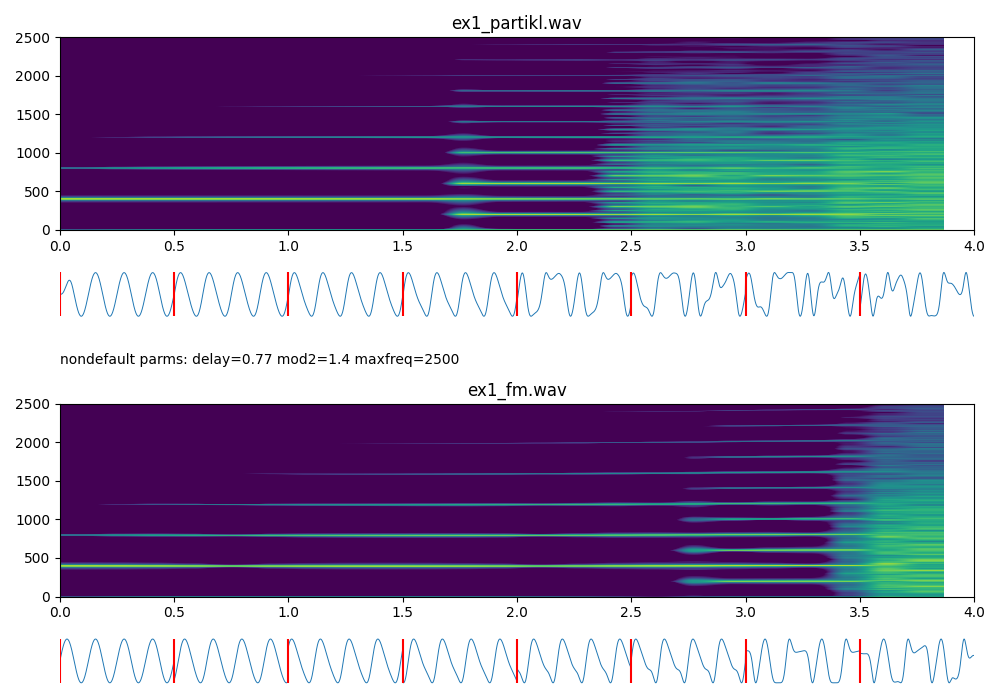
\includegraphics[width=.95\textwidth]{ex1_compare.png}
	\caption{Creating a similar FM feedback sound with the oscillator model and granular model}
	\label{fig:ex1}
\end{figure}

The synthesis models use a set of default parameters shown in listing \ref{lst:defaultparameters} at the very end of the paper, parameter settings deviating from the default setting are listed directly in the figure as nondefault parameters (in between the plots for the granular and oscillator models). The plots show a spectrogram and also zoomed-in snapshots of the waveform at selected locations. The waveform display shows 4 cycles of the waveform in each snapshot, with snapshots being taken every 0.5 seconds of the sound.

In our second example, we will look at the effect of phase delay and how the granular model has a better ability to create a stable pitch regardless of FM feedback modulation artifacts. In the previous example, we used a phase delay that would minimize pitch drift. Here we will try a different phase delay. The oscillator model pitch drift sets in relatively early (before 1 second) in the example sound, while the granular model keeps a steady pitch throughout. The pitch stability of the granular model relates to the steady grain rate, as explained above. The waveform shape can be modulated without affecting the strictly periodic placement of grains. 

\begin{figure}[h]
	\centering
	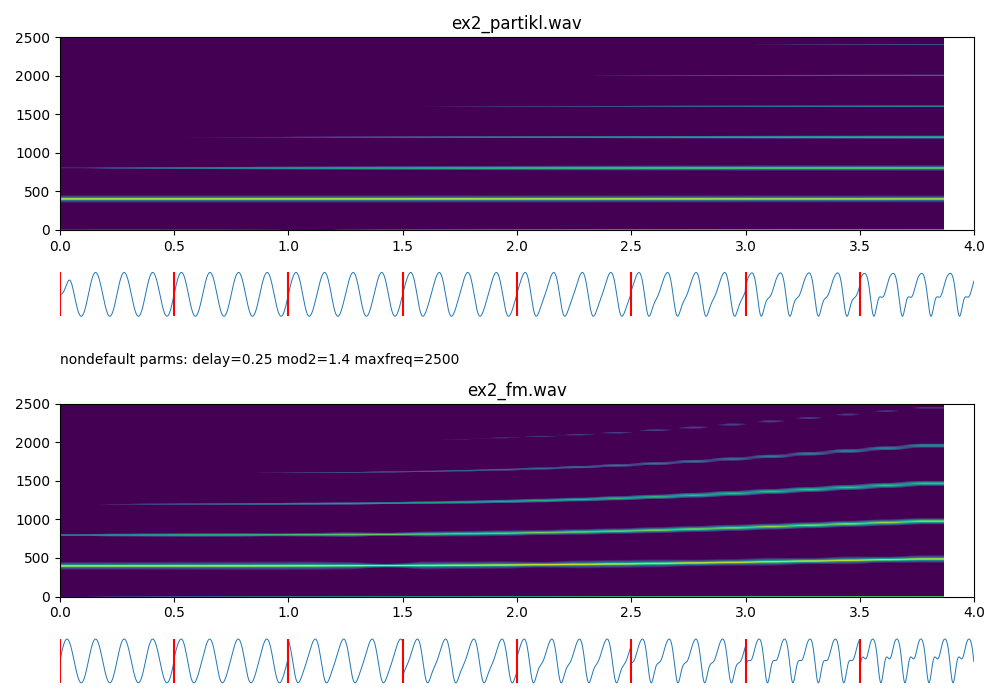
\includegraphics[width=.95\textwidth]{ex2_compare.png}
	\caption{Comparing pitch stability in the two synthesis models}
	\label{fig:ex2}
\end{figure}

In our third example we try to add amplitude modulation to the feedback path to minimize oscillator pitch drift, as can be learned from \cite{Lazzarini-2024}. We keep the phase delay value used in example 2 for comparison. As seen in figure \ref{fig:ex3}, the oscillator model keeps a steady pitch (up until mod index $> 1.0$) and also an even spacing of modulation sidebands throughout the example. The granular model displays a splitting of sidebands into subharmonics at half the fundamental frequency (at 3.3 seconds, where the mod index is approximately 1.15). From this we can assume that the AM in the feedback signal has a different effect in granular than what it has in the oscillator model. The effect of AM in the oscillator model is a more controlled situation, with pitch stability and a constant distance between modulation sidebands. In the granular model, the amplitude modulation has a lesser stabilizing effect. This might relate to the fact that the granular model already has a form of amplitude modulation inherent in the envelope for each grain.

We do note that the oscillator model is not pitch stable at modulation index above 1.0. For values beyond that range, the feedback expression cannot define the waveform uniquely as a function of time, as it has been shown in the analysis of an equivalent phase modulation arrangement \cite[p.61]{Benson}.
The granular model is pitch stable, even if the harmonic pattern makes the fundamental pitch less prominent at high modulation indices. This could indicate that FM feedback in granular synthesis can be utilized to explore new areas of pitch stable FM feedback with high modulation indices.

\begin{figure}[h]
	\centering
	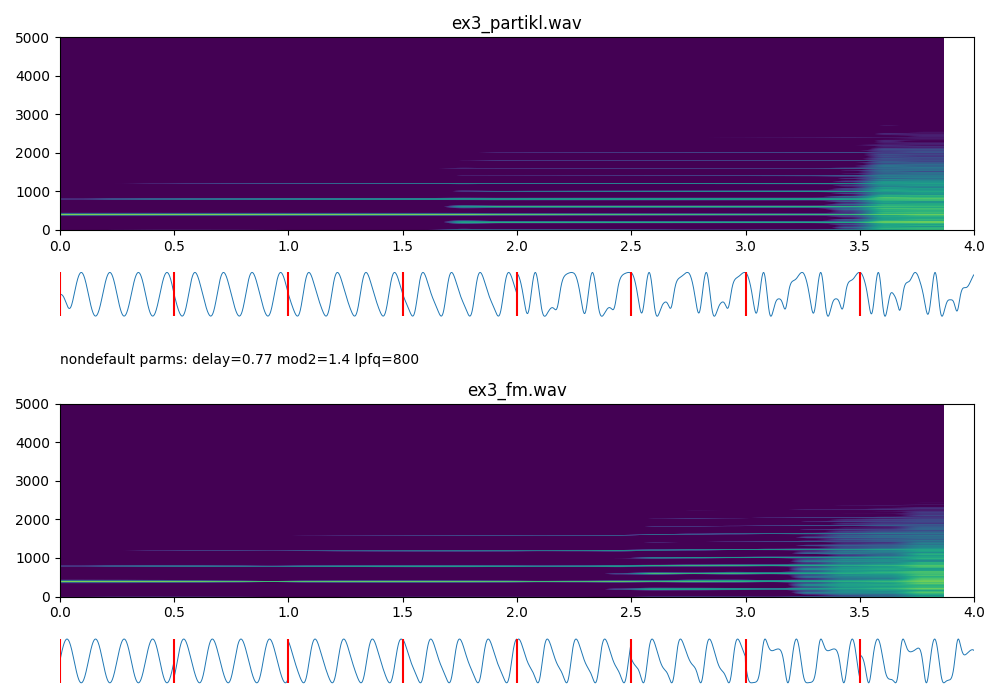
\includegraphics[width=.95\textwidth]{ex3_compare.png}
	\caption{Adding amplitude modulation to the feedback path}
	\label{fig:ex3}
\end{figure}

Adding a lowpass filter to the feedback path can help moderate the chaotic behavior at high modulation indices. As we see in figure \ref{fig:ex4}, it also lower the amplitude of the higher partials generated. For this example we use the same delay value as in example 1, because of the better pitch stability in the oscillator model.  An interesting observation is that the sidebands at half the fundamental frequency appears \emph{earlier} with the oscillator model, as compared with the nonfiltered example (figure \ref{fig:ex1}), and we also see a sudden pitch shift occuring at the same time. In the granular model, those sidebands occur at roughly the same time (same modulation index) in the unfiltered and the lowpass example provided here. Chaotic bahaviour occurs slightly later with lowpass filtering in the granular model. Pitch is stable throughout the granular example.

\begin{figure}[h]
	\centering
	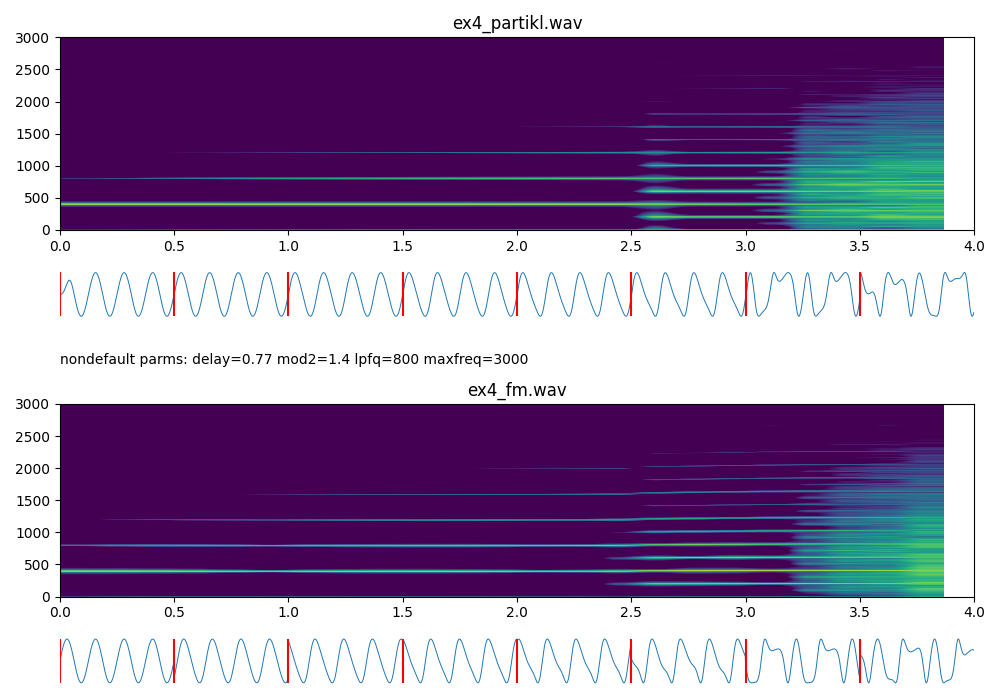
\includegraphics[width=.95\textwidth]{ex4_compare.png}
	\caption{Lowpass filtering the feedback path}
	\label{fig:ex4}
\end{figure}

Another method to moderate chaotic behavior with FM feedback is to add a highpass filter in the feedback path. This will alleviate the effect of DC components resulting from the frequency modulation sideband at 0Hz.  As can be seen in figure \ref{fig:ex5},  it allows higher modulation index before chaotic behavior in the granular model. Interestingly, using the highpass filter creates clearly defined sidebands at further subdivisions (roughly 1/4) of the fundamental frequency. The upper sidebands of the oscillator model show a pitch fluctuation (not prominent in the lower sidebands).

\begin{figure}
	\centering
	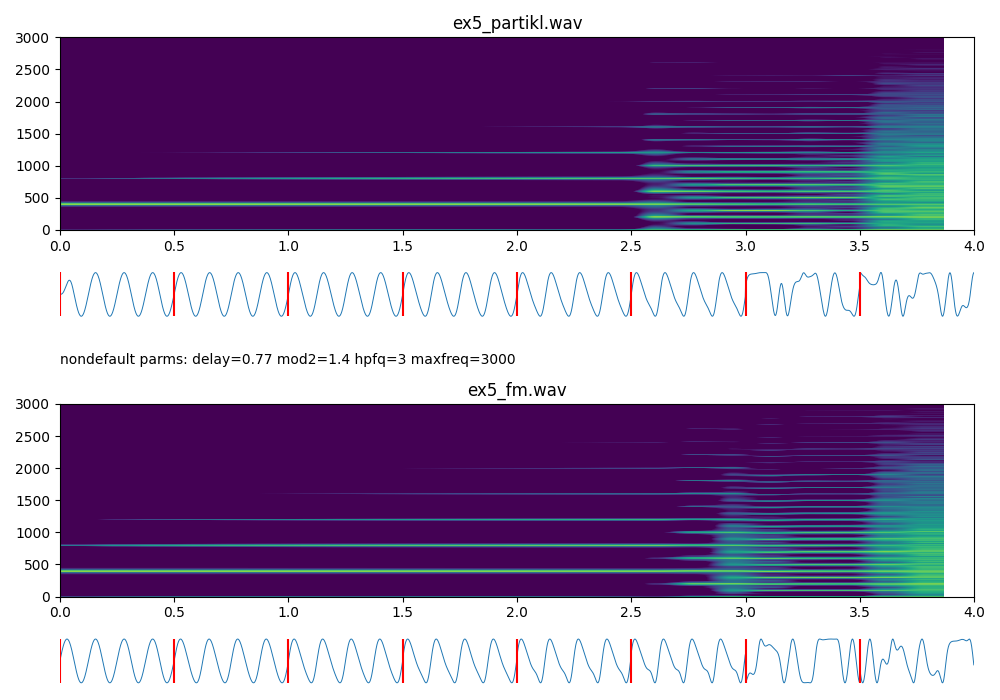
\includegraphics[width=.95\textwidth]{ex5_compare.png}
	\caption{High pass filtering the feedback path.}
	\label{fig:ex5}
\end{figure}

\subsection{Notes}
Take note that some of the effects described are very specific to the parameter settings used. The result may be quite different with slight variation of parameter values. Also note that using a different start value for modulation index will change the behavior: Not surprisingly, the feedback behavior depends on previous values, that is, the current waveform (at any time) is a result of previous feedback, and as such, a different evolution (over time) of e.g. modulation index will lead to different sonic result (at the same modulation index value). To rephrase: the sonic result of any modulation index value depends on previous values of the modulation index. This leads to a pretty rich variety of potential outcomes, and we are currently unsure of how to relate this in a stringent manner when trying to describe specific effects of particular parameter settings.
We have observed a tendency for the complexity of timbre to oscillate slightly with monotonically increasing modulation index. This phenomenon has been observed both with the granular and the oscillator model. Complexities in the sound might occur, and then subside again when increasing the modulation index further by small amounts. This in particular might be an area of further exploration, as it provides rich timbres balancing \emph{"on the edge of chaos"} so to speak. 
 
Regarding filters and delay, it should be mentioned that a filter in the feedback path also will induce delay. We have attempted to compensate for this filter delay in the implementation used for the examples in this paper. The filter delay is frequency dependent, but the delay compensation used here is effective for all frequencies. The required delay time has been calculated from the phase delay at the fundamental frequency of the synthesis example. One should note that some of the artifacts observed might stem from slight variations in phase delay at frequencies corresponding to sideband frequencies. 
Adjusting the phase delay of the feedback loop has significant effect on both the timbral evolution and the pitch stability. Notably, it is possible to find areas of phase delay (e.g. around 0.21 and 0.77) that produce almost pitch stable results even with the traditional oscillator model. We also observe almost identical modulation behavior when adding a whole cycle to the delay time, e.g. very similar results at 1.77 as we see at 0.77. This phenomenon should be investigated further, as it seems the literature shows little previous research on the matter.

\section{Running the provided code examples}
The code examples for this paper can be found in a github repository at \url{https://github.com/Oeyvind/partikkel_fm}. There are Csound orchestra files for FM with granular synthesis and with regular oscillators. To compare the two techniques, it is useful to run both with the same set of parameters (adding only a few extra parameters for granular synthesis), and then compare the generated sound files. The repo contains python files to write score files and render sound with both techniques. This will also display spectrograms for the two generated sound files. The Python files contain default parameter settings as a starting point, and allow parameter modification via command line arguments. For example:
\begin{lstlisting}
python generate_and_compare.py filename cps=200 gr.rate=200
\end{lstlisting}
will modify the fundamental frequency (cps) by setting it to 200Hz, then render sound with both synthesis techniques and display spectrograms for both generated sound files. 

The github repo also contains a granular FM feedback synthesizer instrument (\emph{partikkel\_fm\_feed\_full.csd}) written as a Cabbage plugin with a GUI that allow the user parametric exploration of the technique.

\section{Conclusion}
We have explored a combination of FM feedback with granular synthesis by attempting an as close as possible comparison with regular oscillator FM with feedback. This shows some promising avenues of further exploration, both sonically and theoretically. The tools used for exploration are available in a github repo, encouraging the reader to dive deeper into parametric combinations not yet described here.



%\pagebreak
\begin{thebibliography}{99}

\bibitem{Chowning-73} Chowning, J. (1973). \emph{The synthesis of complex audio spectra by means of frequency modulation.} Journal of the Audio Engineering Society, 21 (7), 527-534.
	
\bibitem{Lazzarini-2024} Lazzarini, V. and Timoney, J. (2024) \emph{Theory and Practice of Higher-Order Frequency Modulation Synthesis.} Journal of New Music Research, 1–16. https://doi.org/10.1080/09298215.2024.2312236

\bibitem{Ervik-Brandtsegg} Ervik, K. and Brandtsegg, Ø. (2013) \emph{Combining granular synthesis with frequency modulation}. Proceedings of the 2013 Linux Audio Conference. \url{http://lac.linuxaudio.org/2013/papers/42.pdf}

\bibitem{Roads-2001} Roads, C. (2001) \emph{Mocrosound}. MIT Press.  ISBN 0-262-18215-7

\bibitem{Brandtsegg-particle} Brandtsegg, Ø. and Saue, S. and Johansen, T. (2011) \emph{Particle synthesis–a unified model for granular synthesis}. Proceedings of the 2011 Linux Audio Conference. \url{http://lac.linuxaudio.org/2011/papers/39.pdf}

\bibitem{Benson} Benson, D. (1986).\emph{ Music: Mathematical Offering}, Oxford Univ. Press.

\bibitem{Cabbage-url} Walsh, R. \emph{Cabbage - A framework for audio software development.} \url{https://cabbageaudio.com}

\bibitem{Lazzarini-2016} Lazzarini, V. et al. (2016). \emph{Csound: A Sound and Music Computing System.} Springer.



\end{thebibliography}


\noindent\begin{minipage}{\linewidth}
\begin{lstlisting}[caption=Default parameters for the synthesis models, label=lst:defaultparameters]
  "dur" = 4 # duration of the generated sound
  "amp" = -6 # overall amplitude
  "cps" = 400 # fundamental frequency 
  "mod1" = 0 # modulation index at start of sound
  "mod2" = 1.5 # modulation index at end of sound
  "delay" = 0 # phase delay for the feedback modulator
  "lpfq" = 21000 # lowpass filter frequency in feedback path
  "hpfq" = 0 #high pass filter frequency in feedback path
  "am" = 0 # enable amplitude modulation in feedback path
  "gr.pitch" = 400 # grain frequency 
  "gr.dur" = 1.5 # grain duration relative to grain rate
  "adratio" = 0.5 # attack to decay ratio of grain envelope
  "sustain" = 0.33 # sustain length for the grain envelope
  "index_map" = 1 # mod index empirical scaling for granular
  "inv_phase2" = 0 # invert the phase of every second grain
\end{lstlisting}
\emph{Comments to the default parameters: "cps" sets the fundamental frequency of the oscillator model, and similarly sets the grain rate for the granular model. The filters in the feedback path are completely bypassed when the cutoff frequency is near the extreme setting. This switch has been set to 20kHz for the lowpass filter, and 0.1Hz for the hipass filter. The parameters "gr.pitch", "gr.dur", "adratio", "sustain", "index\_map" and "inv\_phase2" are only used for the granular model. The "index\_map" parameter implements an empirical compensation of the effect grain duration can have on the effective modulation index. Longer grains (overlapping) will lead to a higher amplitude for the feedback signal. The "inv\_phase2" parameter attempts to implement a granular equivalent of the effect that bipolar amplitude modulation can have on the feedback signal, by inverting the phase of every second grain. For this to work correctly, it also doubles the grain rate (thus also halving the grain duration), so it takes two successive grains to synthesize one duty cycle of the waveform.}
	
\end{minipage}


\end{document}
